\documentclass{article}\usepackage[]{graphicx}\usepackage[]{xcolor}
% maxwidth is the original width if it is less than linewidth
% otherwise use linewidth (to make sure the graphics do not exceed the margin)
\makeatletter
\def\maxwidth{ %
  \ifdim\Gin@nat@width>\linewidth
    \linewidth
  \else
    \Gin@nat@width
  \fi
}
\makeatother

\definecolor{fgcolor}{rgb}{0.345, 0.345, 0.345}
\newcommand{\hlnum}[1]{\textcolor[rgb]{0.686,0.059,0.569}{#1}}%
\newcommand{\hlsng}[1]{\textcolor[rgb]{0.192,0.494,0.8}{#1}}%
\newcommand{\hlcom}[1]{\textcolor[rgb]{0.678,0.584,0.686}{\textit{#1}}}%
\newcommand{\hlopt}[1]{\textcolor[rgb]{0,0,0}{#1}}%
\newcommand{\hldef}[1]{\textcolor[rgb]{0.345,0.345,0.345}{#1}}%
\newcommand{\hlkwa}[1]{\textcolor[rgb]{0.161,0.373,0.58}{\textbf{#1}}}%
\newcommand{\hlkwb}[1]{\textcolor[rgb]{0.69,0.353,0.396}{#1}}%
\newcommand{\hlkwc}[1]{\textcolor[rgb]{0.333,0.667,0.333}{#1}}%
\newcommand{\hlkwd}[1]{\textcolor[rgb]{0.737,0.353,0.396}{\textbf{#1}}}%
\let\hlipl\hlkwb

\usepackage{framed}
\makeatletter
\newenvironment{kframe}{%
 \def\at@end@of@kframe{}%
 \ifinner\ifhmode%
  \def\at@end@of@kframe{\end{minipage}}%
  \begin{minipage}{\columnwidth}%
 \fi\fi%
 \def\FrameCommand##1{\hskip\@totalleftmargin \hskip-\fboxsep
 \colorbox{shadecolor}{##1}\hskip-\fboxsep
     % There is no \\@totalrightmargin, so:
     \hskip-\linewidth \hskip-\@totalleftmargin \hskip\columnwidth}%
 \MakeFramed {\advance\hsize-\width
   \@totalleftmargin\z@ \linewidth\hsize
   \@setminipage}}%
 {\par\unskip\endMakeFramed%
 \at@end@of@kframe}
\makeatother

\definecolor{shadecolor}{rgb}{.97, .97, .97}
\definecolor{messagecolor}{rgb}{0, 0, 0}
\definecolor{warningcolor}{rgb}{1, 0, 1}
\definecolor{errorcolor}{rgb}{1, 0, 0}
\newenvironment{knitrout}{}{} % an empty environment to be redefined in TeX

\usepackage{alltt}
\usepackage[margin=1.0in]{geometry} % To set margins
\usepackage{amsmath}  % This allows me to use the align functionality.
                      % If you find yourself trying to replicate
                      % something you found online, ensure you're
                      % loading the necessary packages!
\usepackage{amsfonts} % Math font
\usepackage{fancyvrb}
\usepackage{hyperref} % For including hyperlinks
\usepackage[shortlabels]{enumitem}% For enumerated lists with labels specified
                                  % We had to run tlmgr_install("enumitem") in R
\usepackage{float}    % For telling R where to put a table/figure
\usepackage{natbib}        %For the bibliography
\bibliographystyle{apalike}%For the bibliography
\IfFileExists{upquote.sty}{\usepackage{upquote}}{}
\begin{document}


\begin{enumerate}
%%%%%%%%%%%%%%%%%%%%%%%%%%%%%%%%%%%%%%%%%%%%%%%%%%%%%%%%%%%%%%%%%%%%%%%%%%%%%%%%
%%%%%%%%%%%%%%%%%%%%%%%%%%%%%%%%%%%%%%%%%%%%%%%%%%%%%%%%%%%%%%%%%%%%%%%%%%%%%%%%
% Question 1
%%%%%%%%%%%%%%%%%%%%%%%%%%%%%%%%%%%%%%%%%%%%%%%%%%%%%%%%%%%%%%%%%%%%%%%%%%%%%%%%
%%%%%%%%%%%%%%%%%%%%%%%%%%%%%%%%%%%%%%%%%%%%%%%%%%%%%%%%%%%%%%%%%%%%%%%%%%%%%%%%
\item A group of researchers is running an experiment over the course of 30 months, 
with a single observation collected at the end of each month. Let $X_1, ..., X_{30}$
denote the observations for each month. From prior studies, the researchers know that
\[X_i \sim f_X(x),\]
but the mean $\mu_X$ is unknown, and they wish to conduct the following test
\begin{align*}
H_0&: \mu_X = 0\\
H_a&: \mu_X > 0.
\end{align*}
At month $k$, they have accumulated data $X_1, ..., X_k$ and they have the 
$t$-statistic
\[T_k = \frac{\bar{X} - 0}{S_k/\sqrt{n}}.\]
The initial plan was to test the hypotheses after all data was collected (at the 
end of month 30), at level $\alpha=0.05$. However, conducting the experiment is 
expensive, so the researchers want to ``peek" at the data at the end of month 20 
to see if they can stop it early. That is, the researchers propose to check 
whether $t_{20}$ provides statistically discernible support for the alternative. 
If it does, they will stop the experiment early and report support for the 
researcher's alternative hypothesis. If it does not, they will continue to month 
30 and test whether $t_{30}$ provides statistically discernible support for the
alternative.

\begin{enumerate}
  \item What values of $t_{20}$ provide statistically discernible support for the
  alternative hypothesis?
  
\begin{knitrout}
\definecolor{shadecolor}{rgb}{0.969, 0.969, 0.969}\color{fgcolor}\begin{kframe}
\begin{alltt}
\hldef{alpha} \hlkwb{=} \hlnum{0.05}
\hldef{n.20} \hlkwb{=} \hlnum{20}

\hldef{(t.20} \hlkwb{=} \hlkwd{qt}\hldef{(}\hlnum{1} \hlopt{-} \hldef{alpha, n.20}\hlopt{-}\hlnum{1}\hldef{))}
\end{alltt}
\begin{verbatim}
[1] 1.729133
\end{verbatim}
\end{kframe}
\end{knitrout}

The built in \texttt{qt()} function makes answering this question simple. It shows that a t value greater than approximately 1.729 with 19 degrees of freedom will get a p-value $<$ $\alpha$ (0.05). \\
  
  \item What values of $t_{30}$ provide statistically discernible support for the
  alternative hypothesis?
  
\begin{knitrout}
\definecolor{shadecolor}{rgb}{0.969, 0.969, 0.969}\color{fgcolor}\begin{kframe}
\begin{alltt}
\hldef{n.30} \hlkwb{=} \hlnum{40}

\hldef{(t.30} \hlkwb{=} \hlkwd{qt}\hldef{(}\hlnum{1} \hlopt{-} \hldef{alpha, n.30}\hlopt{-}\hlnum{1}\hldef{))}
\end{alltt}
\begin{verbatim}
[1] 1.684875
\end{verbatim}
\end{kframe}
\end{knitrout}
This code shows that a t value greater than approximately 1.685 with 29 degrees of freedom will get a p-value $<$ $\alpha$ (0.05). \\

  \item Suppose $f_X(x)$ is a Laplace distribution with $a=0$ and $b=4.0$.
  Conduct a simulation study to assess the Type I error rate of this approach.\\
  \textbf{Note:} You can use the \texttt{rlaplace()} function from the \texttt{VGAM}
  package for \texttt{R} \citep{VGAM}.
  


  
\begin{knitrout}
\definecolor{shadecolor}{rgb}{0.969, 0.969, 0.969}\color{fgcolor}\begin{kframe}
\begin{alltt}
\hldef{sims} \hlkwb{=} \hlnum{10000}
\hldef{err} \hlkwb{=} \hlnum{0}
\hlkwd{set.seed}\hldef{(}\hlnum{7272}\hldef{)}

\hlkwa{for} \hldef{(i} \hlkwa{in} \hlnum{1}\hlopt{:}\hldef{sims)\{}
  \hldef{lap} \hlkwb{=} \hlkwd{rlaplace}\hldef{(}\hlkwc{n} \hldef{=} \hlnum{30}\hldef{,} \hlkwc{location} \hldef{=} \hlnum{0}\hldef{,} \hlkwc{scale} \hldef{=} \hlnum{4}\hldef{)}
  \hldef{lap.20} \hlkwb{=} \hldef{lap[}\hlnum{1}\hlopt{:}\hlnum{20}\hldef{]}
  \hldef{t.sim.20} \hlkwb{=} \hlkwd{mean}\hldef{(lap.20)}\hlopt{/}\hldef{(}\hlkwd{sd}\hldef{(lap.20)}\hlopt{/}\hlkwd{sqrt}\hldef{(n.20))}
  \hldef{t.sim.30} \hlkwb{=} \hlkwd{mean}\hldef{(lap)}\hlopt{/}\hldef{(}\hlkwd{sd}\hldef{(lap)}\hlopt{/}\hlkwd{sqrt}\hldef{(n.30))}

  \hlkwa{if}\hldef{((t.sim.20} \hlopt{>} \hldef{t.20)} \hlopt{&} \hldef{(t.sim.30} \hlopt{<} \hldef{t.30))\{}
    \hldef{err} \hlkwb{=} \hldef{err} \hlopt{+} \hlnum{1}
  \hldef{\}}
\hldef{\}}

\hldef{(t1.err} \hlkwb{=} \hldef{err}\hlopt{/}\hldef{sims)}
\end{alltt}
\begin{verbatim}
[1] 0.0198
\end{verbatim}
\end{kframe}
\end{knitrout}

A type 1 error in this situation occurs if the researchers decide to peak at the results early and find a t value greater than 1.729, but if the trial continued for to 30 months they would have gotten a t value less than 1.685. In order to calculate the error rate from this approach I ran a simulation 10,000 times using \texttt{rlaplace()} from \texttt{VGAM}, and counted an error if the previously mentioned error condition was met. This error rate turned out to be 0.0198, which is low enough for researchers to make the decision to check early wihtout worrying about type 1 error.

  \item \textbf{Optional Challenge:} Can you find a value of $\alpha<0.05$ that yields a 
  Type I error rate of 0.05?
\end{enumerate}
%%%%%%%%%%%%%%%%%%%%%%%%%%%%%%%%%%%%%%%%%%%%%%%%%%%%%%%%%%%%%%%%%%%%%%%%%%%%%%%%
%%%%%%%%%%%%%%%%%%%%%%%%%%%%%%%%%%%%%%%%%%%%%%%%%%%%%%%%%%%%%%%%%%%%%%%%%%%%%%%%
% Question 2
%%%%%%%%%%%%%%%%%%%%%%%%%%%%%%%%%%%%%%%%%%%%%%%%%%%%%%%%%%%%%%%%%%%%%%%%%%%%%%%%
%%%%%%%%%%%%%%%%%%%%%%%%%%%%%%%%%%%%%%%%%%%%%%%%%%%%%%%%%%%%%%%%%%%%%%%%%%%%%%%%
  \item Perform a simulation study to assess the robustness of the $T$ test. 
  Specifically, generate samples of size $n=15$ from the Beta(10,2), Beta(2,10), 
  and Beta(10,10) distributions and conduct the following hypothesis tests against 
  the actual mean for each case (e.g., $\frac{10}{10+2}$, $\frac{2}{10+2}$, and 
  $\frac{10}{10+10}$). 
  \begin{enumerate}
    \item What proportion of the time do we make an error of Type I for a
    left-tailed test?
    \item What proportion of the time do we make an error of Type I for a
    right-tailed test?
    \item What proportion of the time do we make an error of Type I for a
    two-tailed test?
    
    \textbf{In order to answer these questions efficiently I created the function below}
\begin{knitrout}
\definecolor{shadecolor}{rgb}{0.969, 0.969, 0.969}\color{fgcolor}\begin{kframe}
\begin{alltt}
\hldef{simulation} \hlkwb{=} \hlkwa{function}\hldef{(}\hlkwc{a}\hldef{,} \hlkwc{b}\hldef{,} \hlkwc{test}\hldef{)\{}
  \hldef{mu} \hlkwb{=} \hldef{(a}\hlopt{/}\hldef{(a}\hlopt{+}\hldef{b))}
  \hldef{err} \hlkwb{=} \hlnum{0}

  \hldef{t} \hlkwb{=} \hlkwd{c}\hldef{()}
  \hldef{mean} \hlkwb{=} \hlkwd{c}\hldef{()}

  \hlkwa{for} \hldef{(i} \hlkwa{in} \hlnum{1}\hlopt{:}\hldef{sims)\{}
    \hlkwd{set.seed}\hldef{(}\hlnum{7272}\hlopt{+}\hldef{i)}
    \hldef{samp} \hlkwb{=} \hlkwd{rbeta}\hldef{(}\hlkwc{n} \hldef{= n,} \hlkwc{shape1} \hldef{= a,} \hlkwc{shape2} \hldef{= b)}
    \hldef{mean[i]} \hlkwb{=} \hlkwd{mean}\hldef{(samp)}

    \hldef{t[i]} \hlkwb{=} \hldef{(mean[i]}\hlopt{-}\hldef{mu)}\hlopt{/}\hldef{(}\hlkwd{sd}\hldef{(samp)}\hlopt{/}\hlkwd{sqrt}\hldef{(n))}
    \hlkwa{if} \hldef{(t[i]} \hlopt{<} \hldef{t.low} \hlopt{&} \hldef{test} \hlopt{==} \hlsng{'left.sided'}\hldef{)\{}
      \hldef{err} \hlkwb{=} \hldef{err} \hlopt{+} \hlnum{1}
    \hldef{\}}\hlkwa{else if} \hldef{(t[i]} \hlopt{>} \hldef{t.high} \hlopt{&} \hldef{test} \hlopt{==} \hlsng{'right.sided'}\hldef{)\{}
      \hldef{err} \hlkwb{=} \hldef{err} \hlopt{+} \hlnum{1}
    \hldef{\}}\hlkwa{else if} \hldef{((t[i]} \hlopt{<} \hldef{t.2.side[}\hlnum{1}\hldef{]} \hlopt{|} \hldef{t[i]} \hlopt{>} \hldef{t.2.side[}\hlnum{2}\hldef{])} \hlopt{&} \hldef{test} \hlopt{==} \hlsng{'two.sided'}\hldef{)\{}
      \hldef{err} \hlkwb{=} \hldef{err} \hlopt{+} \hlnum{1}
    \hldef{\}}
  \hldef{\}}
  \hldef{mu.xbar} \hlkwb{=} \hlkwd{mean}\hldef{(mean)}
  \hlkwd{return}\hldef{(}\hlkwd{list}\hldef{(err}\hlopt{/}\hldef{sims, mu.xbar))}
\hldef{\}}
\end{alltt}
\end{kframe}
\end{knitrout}
    \item How does skewness of the underlying population distribution effect
    Type I error across the test types?

\begin{table}[ht]
\centering
\begin{tabular}{rrrrrrrr}
  \hline
  $\alpha$ & $\beta$ & $\mu$ & $\mu_{\bar{x}}$ & left t error & right t error & two t error \\ 
  \hline
  10 & 2 & 0.8333 & 0.8330 & 0.0303 & 0.0796 & 0.0619 \\ 
  2 & 10 & 0.1667 & 0.1670 & 0.0796 & 0.0303 & 0.0619 \\ 
  10 & 10 & 0.5000 & 0.5001 & 0.0479 & 0.0525 & 0.0512 \\ 
   \hline
\end{tabular}
\caption{Answers parts 1-b}
\end{table}


\begin{figure}[ht]
\centering
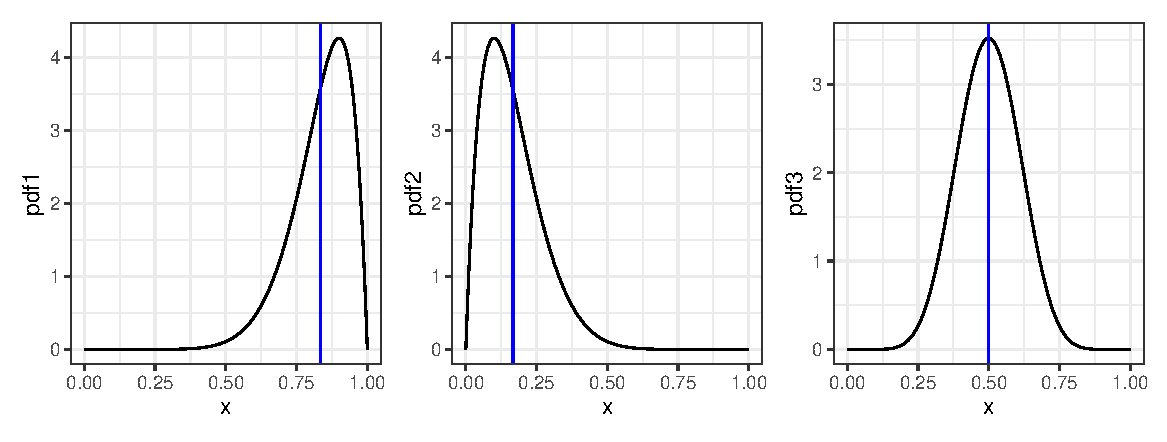
\includegraphics[width = \linewidth]{graphs.pdf}
\end{figure}

  \end{enumerate}
%%%%%%%%%%%%%%%%%%%%%%%%%%%%%%%%%%%%%%%%%%%%%%%%%%%%%%%%%%%%%%%%%%%%%%%%%%%%%%%%
%%%%%%%%%%%%%%%%%%%%%%%%%%%%%%%%%%%%%%%%%%%%%%%%%%%%%%%%%%%%%%%%%%%%%%%%%%%%%%%%
% End Document
%%%%%%%%%%%%%%%%%%%%%%%%%%%%%%%%%%%%%%%%%%%%%%%%%%%%%%%%%%%%%%%%%%%%%%%%%%%%%%%%
%%%%%%%%%%%%%%%%%%%%%%%%%%%%%%%%%%%%%%%%%%%%%%%%%%%%%%%%%%%%%%%%%%%%%%%%%%%%%%%%
\end{enumerate}
\bibliography{bibliography}
\end{document}



@
